\setAuthor{Päivo Simson}
\setRound{piirkonnavoor}
\setYear{2024}
\setNumber{G 10}
\setDifficulty{10}
\setTopic{TODO}

\prob{Põrked}
\begin{wrapfigure}{r}{0.25\textwidth}
\vspace{-25pt}
  \begin{center}
    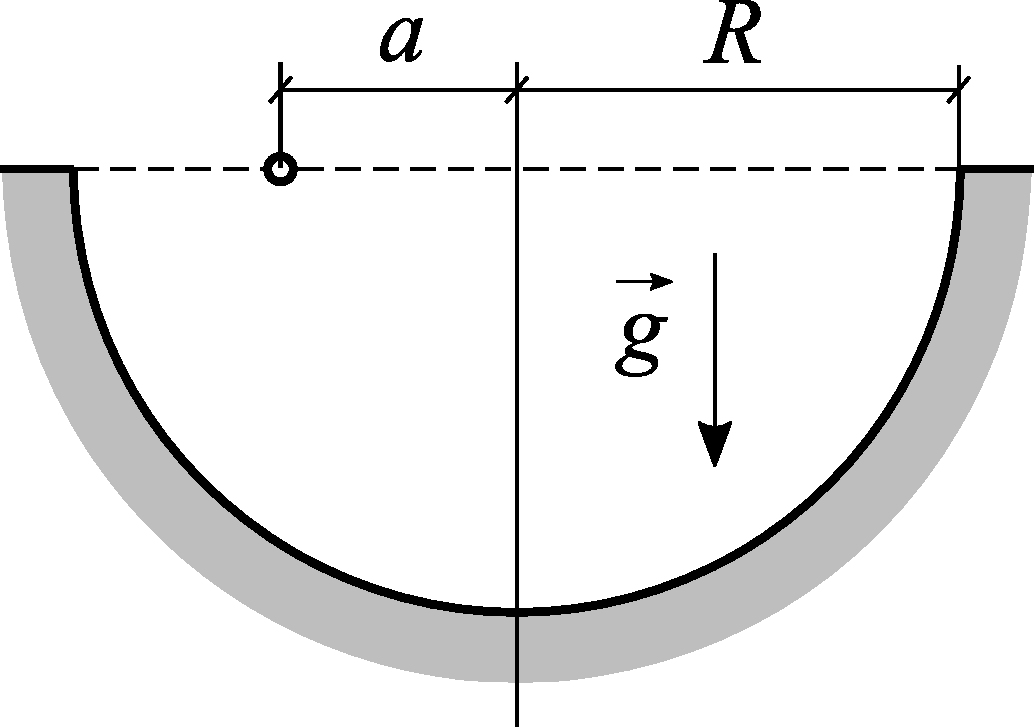
\includegraphics[width=\linewidth]{2024-v2g-10-yl.pdf}
    %\caption{}
  \end{center}
  \vspace{-1cm}
\end{wrapfigure}

Väiksel kummipallil lastakse kukkuda poolkera sisse, mille raadius on $R$. Kõrvaloleval lõikel on näidatud palli algne asukoht, mis on kaugusel $a$ kera tsentrist. Palli algkiirus on null. Leidke üks selline kaugus $a$ ($0<a<R$), mille korral liikumine pärast esimest põrget on perioodiline.


\hint

\solu
\begin{wrapfigure}{r}{0.4\textwidth}
\vspace{-1.1cm}
  \begin{center}
    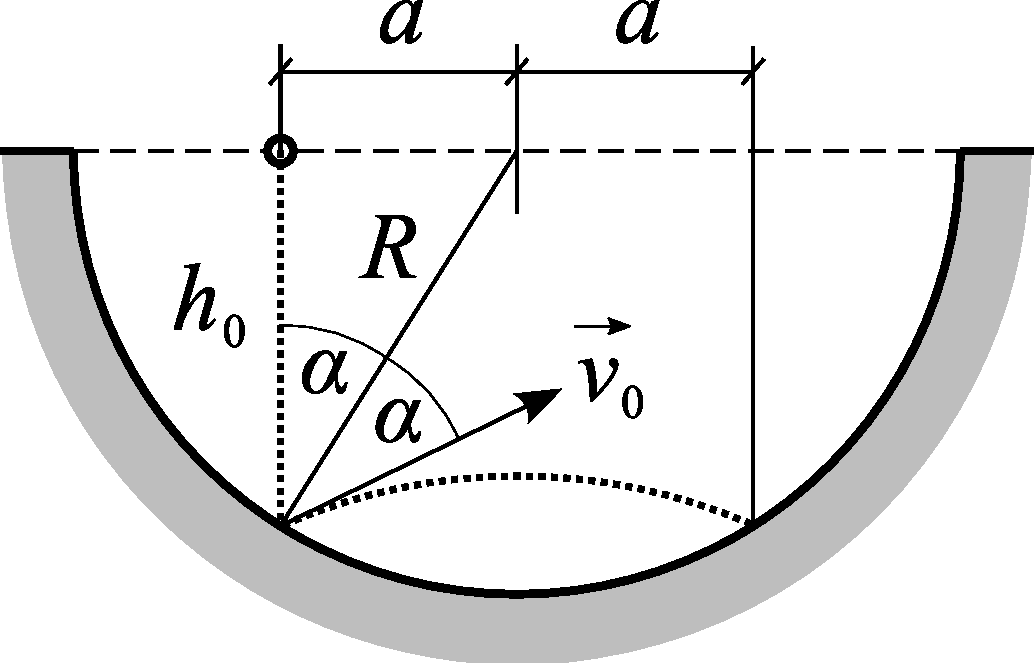
\includegraphics[width=1\linewidth]{2024-v2g-10-yl1.pdf}
  \end{center}
  \vspace{-1cm}
\end{wrapfigure}

\textbf{Lahendus 1}

Ilmselt on lihtsaim perioodiline liikumine selline, mille korral kummipall jääb põrkuma kahe punkti vahel, mis mõlemad on kera keskteljest kaugusel $a$ \p{1}. Uurime, kas selline lahend on võimalik, ja kui on, siis milline peab olema kaugus $a$. 

Kuni esimese põrkeni langeb pall vabalt kõrguse $h_0=\sqrt{R^2-a^2}$ võrra ja saavutab kiiruse $v_0=\sqrt{2gh_0}$ \p{1}. Elastne põrge toimub nurga $2\alpha$ all \p{1} ja edasi liigub pall mööda parabooli, mille haripunkt asub poolkera teljel \p{1}. Paraboolil liikudes on algkkiiruseks $\vec v_0$, mis on horisondi suhtes nurga $90^\circ-2\alpha$ all \p{1}. Kiiruse komponentide ajaline sõltuvus kahe põrke vahelisel ajal on
\begin{align*}
    &v_x=v_0\cos(90^\circ-2\alpha)=v_0\sin 2\alpha=const, \qquad\p{1}\\
    &v_y=v_0\sin(90^\circ-2\alpha)-gt=v_0\cos 2\alpha-gt. \qquad\p{1}
%    &x=v_{x}t=v_0t\sin 2\alpha\\
%    &y=v_{0y}t-gt^2/2
\end{align*}
Kui koordinaatide alguseks valida põrkekoht, siis on parabooli haripunktis $x=v_xt_h=a$, kus $t_h$ on haripunkti jõudmiseks kuluv aeg \p{1}. Lisaks on haripunktis $v_y=0$, millest saame
$t_h=v_0\cos 2\alpha/g$ \p{1}. Võrdus $a=v_xt_h$ annab nüüd
\[a=\frac{v_0^2\sin2\alpha\cos 2\alpha}{g}=2h_0\sin2\alpha\cos 2\alpha\qquad \p{1}\]
Jagame selle võrduse $h_0$-ga ja teisendame saadava võrduse paremat ja vasakut poolt:
\begin{align*}
a/h_0&=2\sin2\alpha\cos 2\alpha\\
\tan\alpha&=4\sin\alpha\cos\alpha(\cos^2\alpha-\sin^2\alpha)\\
\sin\alpha/\cos\alpha&=4\sin\alpha\cos\alpha(1-2\sin^2\alpha)\qquad \p{1}\\
\end{align*}
Saime võrrandi nurga $\alpha$ leidmiseks. Et $\alpha=0$ vastab juhule $a=0$, siis see lahend meile ei sobi. Korrutades viimast võrdust koosinusega ja jagades siinusega saame
\[1=4\cos^2\alpha(1-2\sin^2\alpha)=4(1-\sin^2\alpha)(1-2\sin^2\alpha)\]
Tähistame $x=\sin\alpha$, viime liikmed ühele poole võrdusmärki ja litsustame.
\[4(1-x^2)(1-2x^2)-1=0,\]
\[8x^4-12x^2+3=0.\qquad \p{2}\]
Saime ruutvõrrandi $x^2$ suhtes, mille lahend on
\[x^2=\frac{12\pm\sqrt{12^2-4\cdot8\cdot3}}{16}=\frac{12\pm\sqrt{48}}{16}=\frac{3\pm\sqrt{3}}{4}.\]
Plussiga lahend ei sobi, sest $\sin\alpha$ ei saa olla ühest suurem. Järelikult
\[x=\sin\alpha=\frac{\sqrt{3-\sqrt{3}}}{2},\]
ehk
\[a=R\frac{\sqrt{3-\sqrt{3}}}{2}\approx\num{0.563}R.\qquad \p{1}\]
Näeme, et kahe punkti vahel põrkuv liikumine on võimalik ja see realiseerub ülaltoodud $a$ väärtuse korral. Täpsemalt liigub pall ülevalt alla, siis mööda parabooli paremale, siis vertikaalselt üles ja alla, siis mööda parabooli tagasi esimese põrke punkti, uuesti üles ja alla jne.

\textbf{Lahendus 2}

Eeldame, et lihtsaim perioodiline liikumine on selline, mille korral kummipall jääb põrkuma kahe punkti vahel, mis mõlemad on kera keskteljest kaugusel $a$ \p{1}. Kuni esimese põrkeni langeb pall vabalt kõrguse $h_0$ võrra. Elastne põrge toimub nurga $2\alpha$ all \p{1} ja edasi liigub pall mööda parabooli, mille haripunkt asub eelduse põhjal poolkera teljel \p{1}.

\begin{wrapfigure}{r}{0.6\textwidth}
\vspace{-1.1cm}
  \begin{center}
    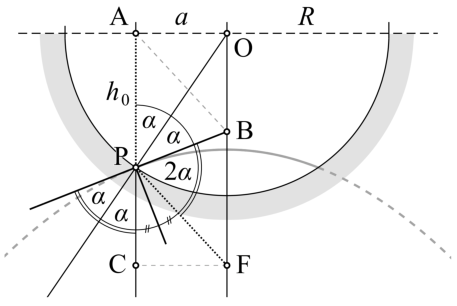
\includegraphics[width=1\linewidth]{2024-v2g-10-yl2.pdf}
  \end{center}
  \vspace{-0.5cm}
\end{wrapfigure}

Parabooli omadustest on teada, et vertikaalne kiir $CP$ peegeldub parabooli fookusesse $F$ \p{2}. Et langemisnurk ja peegeldumisnurk on võrdsed \p{1}, siis järelikult $\angle{FPB}=2\alpha$ \p{1}. Kolmnurgad $PAB$ ja $PBF$ on sarnased, järelikult lõik $PF=h_0$ \p{1} (seega on punkti $O$ läbiv horisontaaljoon parabooli juhtjooneks). Kolmnurgast $POA$ saame
\[\frac{a}{h_0}=\tan\alpha\qquad \p{1}\]
ja kolmnurgast $PCF$
\[\frac{a}{h_0}=\sin(180^\circ-4\alpha)=\sin(4\alpha). \qquad \p{1}\]
Tulemuseks on võrrand $\tan\alpha=\sin 4\alpha$, ehk
\[\frac{\sin\alpha}{\cos\alpha}=4\sin\alpha\cos\alpha(1-2\sin^2\alpha), \qquad \p{1}\]
mille lahendamisel saame (vt lahendus 1)
\[\sin\alpha=\frac{\sqrt{3-\sqrt{3}}}{2}=\frac{a}{R}. \qquad \p{3}\]
\probend